% This work is licensed under the Creative Commons
% Attribution-NonCommercial-ShareAlike 4.0 International License. To view a copy
% of this license, visit http://creativecommons.org/licenses/by-nc-sa/4.0/ or
% send a letter to Creative Commons, PO Box 1866, Mountain View, CA 94042, USA.

% (c) Eric Kunze, 2019

%%%%%%%%%%%%%%%%%%%%%%%%%%%%%%%%%%%%%%%%%%%%%%%%%%%%%%%%%%%%%%%%%%%%%%%%%%%%
% Template for lecture notes and exercises at TU Dresden.
%%%%%%%%%%%%%%%%%%%%%%%%%%%%%%%%%%%%%%%%%%%%%%%%%%%%%%%%%%%%%%%%%%%%%%%%%%%%

\documentclass[ngerman, a4paper, 11pt]{report}

\usepackage[ngerman]{babel}
\usepackage{../../texmf/tex/latex/layoutMathTUD}
\usepackage[smallequationskip]{../../texmf/tex/latex/mathworkMathTUD}

\usepackage{../../texmf/tex/latex/mathoperatorsMathTUD}
\usepackage{../../texmf/tex/latex/maththeorems2MathTUD}

\usepackage{../../texmf/tex/latex/titlepageMathTUD}
\usepackage{../../texmf/tex/latex/graphicsMathTUD}

%%%%%%%%%%%%%%%%%%%%%%%%%%%%%%%%%%%%%%%%%%%%%%%%%%%%%%%%%%%%%%%%%%%
%                        TITLE STYLES                             %
%%%%%%%%%%%%%%%%%%%%%%%%%%%%%%%%%%%%%%%%%%%%%%%%%%%%%%%%%%%%%%%%%%%

\usepackage{titlesec}   % change title headings look
\usepackage{chngcntr}   % modify counters
\usepackage{relsize}    % relative font size (smaller[i], larger[i], ...)

\makeatletter
\@ifpackageloaded{opensans}{}{\usepackage[scale=1]{opensans}}
\ifx\osfamily\undefined
    \newcommand*{\osfamily}{\fontfamily{fos}\selectfont}
    \DeclareTextFontCommand{\textos}{\osfamily}
\fi
\makeatother

\newcommand{\titlefont}{\osfamily}
\newcommand{\chaptersize}{\huge}
\newcommand{\sectionsize}{\LARGE}

\renewcommand{\thepart}{\Alph{part}}

% \titleformat{<command>}[<shape>]{<format>}{<label>}{<sep>}{<before-code>}[<after-code>]
% \titlespacing*{<command>}{<left>}{<before-sep>}{<after-sep>}[<right-sep>]

%%%%%%%%% Kapitel * \\ Titel
%\titleformat{\chapter}[display]{\bfseries\titlefont\color{cddarkblue}}{\chaptersize\smaller \chaptername\;\thechapter}{-10pt}{\chaptersize\MakeUppercase}%
%\titlespacing{\chapter}{10pt}{0pt}{10pt}%

%%%%%%%%% like break but additionally framed
\titleformat{\chapter}[frame]{\bfseries\titlefont\color{cddarkblue}}{\enskip \chaptersize \smaller \chaptername\;\thechapter \enskip}{10pt}{\chaptersize\centering\MakeUppercase}%
\titlespacing{\chapter}{0pt}{0pt}{10pt}%


%%%%%%%%% chapter.section
\counterwithin{section}{chapter}%
\titleformat*{\section}{\bfseries\titlefont\sectionsize}%{\thesection}{8pt}{}%
\titlespacing{\section}{0pt}{10pt}{5pt}
\titleformat*{\subsection}{\bfseries\titlefont\sectionsize\smaller}

%%%%%%%%% section.
%\renewcommand{\thechapter}{\Roman{chapter}}
%\titlelabel{\thetitle.\quad} % "." behind section/sub... (3. instead of 3)
%\counterwithout{section}{chapter}%
%\titleformat*{\section}{\bfseries\titlefont\sectionsize}%{\thesection}{8pt}{}%
%\titleformat*{\subsection}{\bfseries\titlefont\sectionsize\smaller}

%%%%%%%%% section
%\titlelabel{\thetitle \quad} % no "." behind section/sub... (3 instead of 3.)
%\titleformat{\section}[hang]{\bfseries\titlefont\sectionsize}{\thesection}{8pt}{}%
%\titleformat*{\section}{\bfseries\titlefont\sectionsize}
%\titleformat*{\subsection}{\bfseries\titlefont\sectionsize\smaller}

%%%%%%%%%%%%%%%%%%%%%%%%%%%%%%%%%%%%%%%%%%%%%%%%%%%%%%%%%%%%%%%%%%%
%                          HIGHLIGHTING                           %
%%%%%%%%%%%%%%%%%%%%%%%%%%%%%%%%%%%%%%%%%%%%%%%%%%%%%%%%%%%%%%%%%%%
\newcommand{\begriff}[1]{\textbf{#1}}
\newcommand{\person}[1]{\textsc{#1}}

%%%%%%%%%%%%%%%%%%%%%%%%%%%%%%%%%%%%%%%%%%%%%%%%%%%%%%%%%%%%%%%%%%%
%                             COUNTER                             %
%%%%%%%%%%%%%%%%%%%%%%%%%%%%%%%%%%%%%%%%%%%%%%%%%%%%%%%%%%%%%%%%%%%
\usepackage{chngcntr}

% automatic reset of section after chapter ended 
\pretocmd{\chapter}{\setcounter{section}{0}}{}{}

% automatic reset of equation counter in each section
\pretocmd{\section}{\setcounter{equation}{0}}{}{}

\counterwithin{themcount}{chapter}

%%%%%%%%%%%%%%%%%%%%%%%%%%%%%%%%%%%%%%%%%%%%%%%%%%%%%%%%%%%%%%%%%%%
%                          ENUMERATIONS                           %
%%%%%%%%%%%%%%%%%%%%%%%%%%%%%%%%%%%%%%%%%%%%%%%%%%%%%%%%%%%%%%%%%%%
\usepackage{enumerate}
\usepackage[inline]{enumitem} 		%customize label

\renewcommand{\labelitemi}{\raisebox{1pt}{\scalebox{.6}{$\blacksquare$}}}
\renewcommand{\labelitemii}{$\vartriangleright$}
\renewcommand{\labelitemiii}{--}
% Variantionen des Dreiecks als Aufzählungszeichen $\blacktriangleright$ / $\vartriangleright$ / $\triangleright$

\renewcommand{\labelenumi}{(\arabic{enumi})}
\renewcommand{\labelenumii}{\alph{enumii}.}
\renewcommand{\labelenumiii}{\roman{enumiii}.}
%%%%%%%%%%%%%%%%%%%%%%%%%%%%%%%%%%%%%%%%%%%%%%%%%%%%%%%%%%%%%%%%%%%


%%%%%%%%%%%%%%%%%%%%%%%%%%%%%%%%%%%%%%%%%%%%%%%%%%%%%%%%%%%%%%%%%%%
%                         HEADER & FOOTER                         %
%%%%%%%%%%%%%%%%%%%%%%%%%%%%%%%%%%%%%%%%%%%%%%%%%%%%%%%%%%%%%%%%%%%
\newcommand*{\rightinfo}{Vorlesung ''Stochastik -- Finanzmathematik`` bei Prof. Dr. Keller-Ressel im Wintersemester 2019/20}

\usepackage{tikz}       % needed for right info
\usetikzlibrary{calc}

\usepackage{fancyhdr} 	% customize header / footer
% Add new page-style (just footer), patch \chapter command to use this page style

\fancypagestyle{myStyle}{%
    \fancyhf{} %
    \fancyfoot[C]{\thepage} %
    \renewcommand{\headrulewidth}{0pt}     % Line at the header invisible
    \renewcommand{\footrulewidth}{0pt}     % Line at the footer visible
    \fancyhead[C]{\textcolor{gray}\leftmark} %
    \fancyhead[R]{%
        \begin{tikzpicture}[overlay,remember picture]
        \node [
        fill=none,  % Farbe des Randstreifens
        text=gray,  % Textfarbe
        font=\osfamily\normalsize,  % Einstellungen für die Schrift
        inner xsep=\footskip,       % Abstand des Textes von unten
        % maximale Textbreite = Papierhöhe - 2*Abstand des Textes von unten:
        text width={\dimexpr\paperheight-2\footskip\relax},
        align=center,
        minimum height=7mm,% Breite des Randstreifens
        anchor=south west,
        rotate=90
        ]
        at ($(current page.south east)+(-10mm,0mm)$)
        {\rightinfo};
        \end{tikzpicture}%
     }
}

\fancypagestyle{rightinfo}{%
    \fancyhf{} %
    \fancyfoot[C]{\thepage} %
    \renewcommand{\headrulewidth}{0pt}     % Line at the header invisible
    \renewcommand{\footrulewidth}{0pt}     % Line at the footer visible
    \fancyhead[R]{%
        \begin{tikzpicture}[overlay,remember picture]
        \node [
        fill=none,  % Farbe des Randstreifens
        text=gray,  % Textfarbe
        font=\sffamily\normalsize,  % Einstellungen für die Schrift
        inner xsep=\footskip,       % Abstand des Textes von unten
        % maximale Textbreite = Papierhöhe - 2*Abstand des Textes von unten:
        text width={\dimexpr\paperheight-2\footskip\relax},
        align=center,
        minimum height=7mm,% Breite des Randstreifens
        anchor=south west,
        rotate=90
        ]
        at ($(current page.south east)+(-10mm,0mm)$)
        {\rightinfo};
        \end{tikzpicture}%
     }
}

%% changes pagestyle on first page of each chapter; instead of empty page the normal footer is printed
\patchcmd{\chapter}{\thispagestyle{plain}}{\thispagestyle{rightinfo}}{}{}

\pagestyle{myStyle}
\pagenumbering{arabic}

%% remember chapter-title in \leftmark and \rightmark
%\renewcommand{\chaptermark}[1]{%
%    \markboth{\chaptername
%        \ \thechapter:\ #1}{}}
%
%% remember section title in \leftmark
%\renewcommand{\sectionmark}[1]{%
%    \markright{\thesection.\ #1}{}}
%
%%change header:
%\renewcommand{\headrulewidth}{0.75pt}
%\renewcommand{\footrulewidth}{0.3pt}
%\lhead{\rightmark}%left: section-number. section-title
%\rhead{\leftmark}%right: chapter chapternumber: chapter-title

% remove page number from part{}-pages
%\let\sv@endpart\@endpart
%\def\@endpart{\thispagestyle{empty}\sv@endpart}
%%%%%%%%%%%%%%%%%%%%%%%%%%%%%%%%%%%%%%%%%%%%%%%%%%%%%%%%%%%%%%%%%%%


%%%%%%%%%%%%%%%%%%%%%%%%%%%%%%%%%%%%%%%%%%%%%%%%%%%%%%%%%%%%%%%%%%%
%                        TABLE OF CONTENTS                        %
%%%%%%%%%%%%%%%%%%%%%%%%%%%%%%%%%%%%%%%%%%%%%%%%%%%%%%%%%%%%%%%%%%%
\usepackage{tocloft}

\renewcommand{\cfttoctitlefont}{\titlefont\Huge\bfseries}
\setcounter{tocdepth}{1}
%%%%%%%%%%%%%%%%%%%%%%%%%%%%%%%%%%%%%%%%%%%%%%%%%%%%%%%%%%%%%%%%%%%

%%%%%%%%%%%%%%%%%%%%%%%%%%%%%%%%%%%%%%%%%%%%%%%%%%%%%%%%%%%%%%%%%%%
%                            LISTINGS                             %
%%%%%%%%%%%%%%%%%%%%%%%%%%%%%%%%%%%%%%%%%%%%%%%%%%%%%%%%%%%%%%%%%%%
\usepackage{listings}


\usepackage{../../texmf/tex/latex/referencesMathTUD}

%%%%%%%%%%%%%%%%%%%%%%%%%%%%%%%%%%%%%%%%%%%%%%%%%%%%%%%%%%%%%%%%%%%%%%%%%%%%

%---------------------------------------
% additional packages
%---------------------------------------

% none

%---------------------------------------
% general settings
%---------------------------------------

\name{Eric Kunze}
\matnr{Nummer}
\email{\href{mailto:eric.kunze@mailbox.tu-dresden.de}{\ttfamily eric.kunze@mailbox.tu-dresden.de}}

\modul{Vertiefung in der Stochastik}
\period{Wintersemester 2019/20}

%\renewcommand{\tutor}{Dr. Legrand}
%\renewcommand{\group}{Tag x. DS, (un)gerade Woche}

\lecturer{Prof. Dr. Martin Keller-Ressel}
\faculty{Mathematik}
\institute{Stochastik}
\professorship{Stoch. Analysis und Finanzmathematik}

%%%%%%%%%%%%%%%%%%%%%%%%%%%%%%%%%%%%%%%%%%%%%%%%%%%%%%%%%%%%%%%%%%%%%%%%%%%%



\undef\folge
\NewDocumentCommand{\folge}{m m}{\left( #1 \right)_{#2}}
\renewcommand{\complement}{\mathsf{C}}

\renewcommand{\F}{\mathcal{F}}
\renewcommand{\G}{\mathcal{G}}

\newcommand{\widesim}[1][2.5]{
	\mathrel{\scalebox{#1}[1]{\ensuremath{\sim}}}
}

\usepackage{mwe}

%%%%%%%%%%%%%%%%%%%%%%%%%%%%%%%%%%%%%%%%%%%%%%%%%%%%%%%%%%%%%%%%%%%%%%%%%%%%


\begin{document}

\makeTUtitle
    
\tableofcontents

\chapter{Einführung}
\label{chapter_1_einfuehrung}
\section{Zentrale Fragestellungen der Finanzmathematik}

\subsection{Bewertung von Derivaten und Abischerung gegen aus deren Kauf/Verkauf entstehende Risiken}

\begin{definition}[Derivat]
	Ein \begriff{Derivat} ist ein Finanzprodukt, dessen Auszahlung sich vom Preis eines oder mehrerer Basisgüter [underlying] ableitet.
\end{definition}

\begin{beispiel}
	\begin{itemize}[nolistsep, leftmargin=*, topsep=-\parskip]
		\item Recht in drei Monaten 100.000 GBP gegen 125.000 EUR zu erhalten (Call-Option; underlying: Wechselkurs GBP in EUR)
		\item Recht innerhalb des nächsten Jahres 100.000 MWh elektrische Energie zum Preis von 30 EUR/MWh zu konsumieren mit Mindestabnahme 50.000 MWh (Swing-Option; underlying: Strompreis)
		\item Kauf- und Verkaufsoptionen azf Aktien (underlying: Aktienkurs)
	\end{itemize}
\end{beispiel}

\textbf{Fragestellungen:}
\begin{itemize}[nolistsep, label=--, topsep=-\parskip]
	\item Was ist der ''faire`` Preis für solch ein Derivat? (''Pricing`` / Bewertung)
	\item Wie kann sich der Verkäufer gegen die eingegangenen Risiken absichern? (''Hedging`` / Absicherung)
\end{itemize}

\subsection{Optimale Investition: Zusammenstellen von nach Risiko-/ Ertragsgesichtspunkten optimalen Portfolios}

\begin{itemize}[nolistsep, leftmargin=*, topsep=-\parskip]
	\item Wie wäge ich Risiko gegen Ertrag ab?
	\item Was bedeutet optimal?
	\item Lösung des resultierenden Optimierungsproblems
\end{itemize}

\subsection{Risikomanagement und Risikomessung}

gesetzliche Vorschriften (Basel und Solvency) sollen Stabilität des Banken- und Versicherungssystems angesichts verschiedener Risiken sicherstellen \\
$\to$ mathematische Theorie der konvexen und kohärenten Risikomaße

\textbf{Mathematische Werkzeuge:} Wahrscheinlichkeitstheorie und stochastische Prozesse (Dynamik in der Zeit), zusätzlich etwas lineare Algebra, Optimierung, Maßtheorie
\section{Mathematisches Finanzmodell}

Wir betrachten
\begin{enumerate}[leftmargin=*]
	\item einen Wahrscheinlichkeitsraum $\Omega, \F, \P)$, später auch weitere Maße $\Q, \dots$ auf demselben Maßraum $(\Omega, \F)$. Die $\omega \in \Omega$ werden als \begriff{Elementarereignisse} oder \begriff{''Szenarien``} bezeichnet.
	\item Zeitachse $I$ entweder $I = \menge{t_1, t_2, \dots t_N = T}$ ($N$-Perioden-Modell; diskretes Modell) oder $I = [O,T]$ (stetiges Modell)
	Dabei wird $T$ als \begriff{Zeithorizont} bezeichnet.
	\begin{definition}[stochastischer Prozess]
		Ein stochastischer Prozess $S$ ist eine messbare Abbildung 
		\begin{equation*}
		\bigabb{S}{(\Omega \times I)}{\Rd}{(\omega, t)}{S_t(\omega)}
		\end{equation*}
	\end{definition}
	Insbesondere ist 
	\begin{itemize}[nolistsep, topsep=-\parskip]
		\item $t \mapsto S_t(\omega)$ eine Funktion $I \to \Rd$ für jedes $\omega \in \Omega$ 
		\item $\omega \mapsto S_t(\omega)$ eine Zufallsvariable $\Omega \to \Rd$ für jedes $t \in I$
	\end{itemize}
	\item ~\vspace{-2em}
	 \begin{definition}[Filtration]
	 	Eine Filtration ist eine Folge von $\sigma$-Alegbren $\folge{\F_t}{t \in I}$ mit der Eigenschaft
	 	\begin{equation*}
	 	\F_s \subseteq \F_t \quad \forall s,t \in I, s \le t \qquad \und \qquad \F_t \subseteq \F \quad \forall t \in I
	 	\end{equation*}
	 \end{definition}
 	\begin{*interpretation}
 		$\F_t$ beschreibt die den Marktteilnehmern zum Zeitpunkt $t$ bekannte bzw. verfügbare Information. Ein Ereignis $A \in \F_t$ gilt als ''zum Zeipunkt $t$ bekannt``.
 	\end{*interpretation}
	
	\begin{*erinnerung_inline}
		Eine $\Rd$-wertige Zufallsvariable $X$ heißt $\F_t$-messbar, wenn
		\begin{equation*}
		X^{-1}(B) \in \F_t \quad \forall \text{ Borelmengen } B \subseteq \Rd
		\end{equation*}
	\end{*erinnerung_inline}

	\begin{beispiel}
		Sei $S$ ein stochastischer Prozess. Dann heißt
		\begin{equation*}
			\F_t^S = \sigma( \menge{(S_r) : r \in I, r \le t} )
		\end{equation*}
		von $S$ erzeugte Filtration.
	\end{beispiel}
	
	\begin{definition}[adaptierter Prozess]
		Ein stochastischer Prozess $\folge{S_t}{t \in I}$ auf $(\Omega, \F)$ heißt \begriff{adapiert} bezüglich einer Filtration $\folge{\F_t}{t \in I}$, wenn gilt $S_t$ ist $\F_t$-messbar für alle $t \in I$.
	\end{definition}
	
	Interpretation: Der Wert $S_t$ ist zum Zeitpunkt $t$ ''bekannt``.
	
	Warum Filtrationen in der Finanzmathematik?
	\begin{itemize}[nolistsep, topsep=-\parskip]
		\item Unterscheidung Zunkunft/Vergangenheit
		\item Unterscheidung Informationen (Insider/Outsider) Unterscheidung Filtration $\folge{\F_t}{t \in I}$ bzw. $\folge{\G_t}{t \in I}$
	\end{itemize}
	
	\item Anlagegüter [assets]: $\R^{d+1}$-wertiger stochastischer Prozess mit Komponenten
	\begin{equation*}
		\bigabb{S^i}{(\Omega \times I)}{\R}{(\omega, t)}{S_t^i(\omega)} \quad (i \in \menge{0, 1, \dots , d})
	\end{equation*}
	$S_t^i$ beschreibt dabei den Preis des $i$-ten Anlageguts zum Zeitpunkt $t$. $S^i$ ($i \in \menge{1, \dots , d}$) ist typischerweise
	\begin{itemize}[nolistsep, topsep=-\parskip]
		\item Aktien [stock], Unternehmensanteil
		\item Währung [currency] bzw. Wechselkurs
		\item Rohstoff [commodity] wie z.B. Öl, Edelmetall, Elektrizität
		\item Anleihe [bond] $\dots$ Schuldverschreibung
	\end{itemize}
	
	Hauptannahme: $S^i$ ist liquide gehandelt (z.B. Börse), d.h. der Kauf und Verkauf zum Preis $S_t^i$ ist jederzeit möglich. 
	Der ''Numeraire`` $S^0$ hat eine Sonderrolle und beschreibt die Verzinsung von nicht in $(S^1, \dots , S^d)$ angelegtem Kapital. Er wird als risikolos betrachtet.
\end{enumerate}

\begin{definition}
	Ein Finanzmarktmodell (FFM) mit Zeitachse $I$ ist gegeben durch
	\begin{enumerate}[nolistsep, topsep=-\parskip]
		\item einen Wahrscheinlichkeitsraum $(\Omega, \F, \P)$ mit Filtration $\folge{\F_t}{t \in I}$
		\item einem an $\folge{\F_t}{t \in I}$ adaptierten, $\R^{d+1}$-wertigen stiochastischen Prozess $S_t = (S_t^0, S_t^1 , \dots , S_t^d)$ mit $t \in I$.
	\end{enumerate}
\end{definition}
\begin{beispiel}[Cox-Ross-Rubinstein-Modell]
	Das CRR-Modell ist ein zeitdiskretes Modell beschrieben durch
	\begin{itemize}[nolistsep, topsep=-\parskip]
		\item $S_n^0 = (1+r)^n$ \dots Verzinsung mit konstanter Rate $r$
		\item $S_n^1 = S_0^1 \prod_{k=1}^n (1+R_k)$, wobei $(R_1, R_2, \dots)$ unabhängige Zufallsvariablen mit zwei möglichen Werten $a < b$ sind
	\end{itemize}

	\begin{tabularx}{\columnwidth}{XX}
		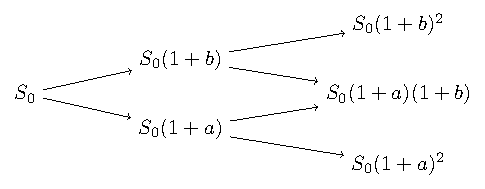
\includegraphics[width=.5\textwidth]{./stochv_abbildungen/stochv_1_2_crr}
		\captionof{figure}{Cox-Ross-Rubinstein-Modell}
		&
		$\hookrightarrow$ rekombinierender Baum, \newline
		Ereignisse $\omega$ entsprechen Pfaden im Baum
	\end{tabularx}	
\end{beispiel}

\begin{beispiel}[Black-Scholes-Modell, zeitstetig]
	Beim Black-Scholes-Modell handelt es sich um ein zeitstetiges Modell auf einem unendlichen Wahrscheinlichkeitsraum.
	\begin{equation*}
		\begin{aligned}
		S_t^0 &= e^{rt} && (\text{Verzinsung mit konstanter Rate } r) \\
		S_t^1 &= S_0^1 * \exp\brackets{(\mu-\frac{\sigma^2}{2}) + \sigma B_t} &&\mit \mu \in \R, \sigma > 0, S_0^1 > 0
		\end{aligned}
	\end{equation*}
	Der Term $\mu-\frac{\sigma^2}{2}$ beschreibt dabei eine Trendkomponenten, $B_t$ eine ''Brownsche Bewegung`` (zeitstetiger Prozess).
	\begin{center}
		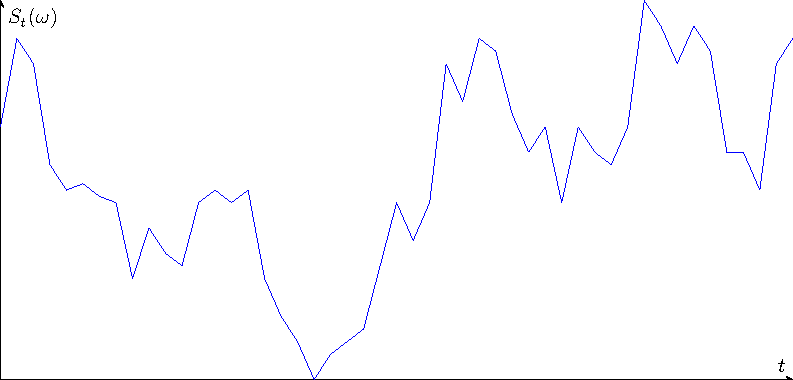
\includegraphics[width=.5\textwidth]{./stochv_abbildungen/stochv_1_2_bsm}
		\captionof{figure}{Black-Scholes-Modell}
	\end{center}
\end{beispiel}


\section{Anleihen und grundlegende Beispiele für Derivate}

Hier betrachten wir immer nur ein Basisgut $S_t = S_t^1$.

\begin{enumerate}[leftmargin=*, label=(\alph*)]
	\item \begriff{Anleihe} [bond] (genauer: Null-Kupon-Anleihe [zero-coupon bond])
	
	Der Emittent (Herausgeber) einer Anleihe mit Endfälligkeit [maturity] $T$ garantiert dem Käufer zum Zeitpunkt $T$ den Betrag $N$ (EUR/USD/...) zu zahlen.
	Typische Emittenten sind z.B. Staaten [government bond] oder Unternehmen (als Alternative zur Kreditaufnahme).
	Nach Emission werden Anleihen auf dem Sekundärmarkt weiterverkauft, d.h. liquide gehandelte Wertpapiere. 
	
	\begin{tabular}{ll}
		Preis bei Emission: & $B(0,T)$ \\
		Preis bei Weiterverkauf zum Zeitpunkt $t \le T$: & $B(t,T)$ \\
	\end{tabular}
	
	Es ist $B(T,T) = N$ und wir normieren stets $N=1 \follows B(T,T)=1$.
	
	Anleihen von West-/ Nord-/ Mitteleuropäischen Staaten und den USA sowie Kanada werden als risikolos betrachtet (sichere Zahlung). Sonst: Kreditrisiko
	
	Risikofreie Anleihen können als Numeraire $S_t^0 = B(t,T)$ genutzt werden.
	
	\begin{center}
		%TODO BILD (1)
		\includegraphics[width=.5\textwidth]{example-image}
		\captionof{figure}{Zahlungsstrom einer Anleihe}
	\end{center}
	
	\item \begriff{Terminvertrag} [forward contract]
	
	aus Käufersicht: Vereinbarung zu bestimmtem zukünftigen Zeitpunkt $T$ eine Einheit des Basisguts $S$ zum Preis $K$ zu kaufen (Kaufverpflichtung). Beliebt ist dieser bei Rohstoffen und Elektrizität.
	
	Auszahlungsprofil: $F_T = S_T - K$
	Preis zum Zeitpunkt $t$: $F_t$
	
	\begin{center}
		%TODO BILD (2)
		\includegraphics[width=.5\textwidth]{example-image}
		\captionof{figure}{Auszahlungsprofil eines Terminvertrags}
	\end{center}
	
	
	\item \begriff{(Europäische) Put- bzw. Call-Option}
	
	Recht zu einem zukünftigen Zeitpunkt $T$ eine Einheit des Basisguts $S$ zum Preis $K$ zu verkaufen (put) bzw. zu kaufen (call)
	$\to$ keine Kaufverpflichtung !
	% Vergleich zum Terminvertrag: keine Pflicht
	
	Auszahlungsprofil:
	\begin{itemize}
		\item Call: $C_T = \begin{cases} S_T - K & S_T \ge K \\ 0 & S_T < K \end{cases} = \brackets{S_T - K}_+$
		%TODO Bild (3)
		\item Put: $P_T = \begin{cases} 0 & S_T \ge K \\ K - S_T & S_T < K \end{cases} = \brackets{K - S_T}_+$ 
		%TODO Bild (4)
	\end{itemize}

	\item \begriff{Amerikanische Put- bzw. Call-Option}
	
	wie Put/Call, aber mit Ausübung zu beliebigem Zeitpunkt $\tau \in [0,T]$.
	
	\begin{tabular}{ll}
		Preis zum Zeitpunkt $t$: & $P_t^{AM}$, $C_t^{AM}$ \\
		Auszahlungsprofil zum Zeitpunkt $\tau$: & $\brackets{S_\tau - K}_+$, $\brackets{K - S_\tau}_+$
	\end{tabular}
	
	Der Zeitpunkt $\tau$ muss im Allgemeinen als Lösung eines stochastischen Optimierungsproblems bestimmt werden (optimales Stopp-Problem).
\end{enumerate}
\section{Elementare Replikations- und Ar"-bitrage"-argumente}

Was können wir (mit elementaren Mitteln) über die ''fairen`` Preise $B(t,T), F_t, C_t, P_t$ aussagen?

Wir verwenden:

\begin{itemize}[topsep=-\parskip]
	\item \begriff{Replikationsprinzip}: zwei identische, zukünftige Zahlungsströme haben auch heute denselben Wert (ein Zahlungsstrom ''repliziert`` den anderen)
	\item \begriff{No-Arbitrage-Prinzip}: ''Ohne Kapitaleinsatz kann kein sicherer Gewinn ohne Verlustrisiko erzielt werden.`` (Arbitrage = risikofreier Gewinn)
	\item \begriff{Superreplikationsprinzip} (schwächere Form des Replikationsprinzips): Ist ein Zahlungsstrom in jedem Fall größer als ein anderer, so hat er auch heute den größeren Wert.
\end{itemize}

\begin{center}
	\begin{tabular}{|c|c|c|}
		\hline
		stark & Replikationsprinzip & eingeschränkt anwendbar \\
		$\downarrow$ & Superreplikationsprinzip & $\uparrow$ \\
		schwach & No-Arbitrage-Prinzip & immer anwendbar \\
		\hline
	\end{tabular}
\end{center}

\begin{lemma} % 1.1
	Für den Preis $C_T$ des europäischen Calls gilt:
	\begin{equation*}
		\brackets{S_t - K B(t,T)}_+ \le C_t \le S_t
	\end{equation*}
\end{lemma}
\begin{proof}
	untere Schranke: Für Widerspruch nehme an, dass $S_t - K B(t,T) - C_t = \epsilon > 0$.
	
	\begin{center}
		\begin{tabular}{|l|c|cc|} % Wert in T über rechte beide Spalten
			\hline \multirow{2}{*}{Portfolio} & \multirow{2}{*}{Wert in $t$} & \multicolumn{2}{c|}{Wert in $T$} \\
			&& $S_T \le K$ & $S_T > K$ \\ \hline \hline
			Kaufe Call & $C_t$ & $0$ & $S_T - K$ \\
			Verkaufe Basisgut & $-S_T$ & $-S_T$ & $-S_T$ \\
			Kaufe Anleihe & $\epsilon + K B(t,T)$ & $\frac{\epsilon}{B(t,T)} + K$ &  $\frac{\epsilon}{B(t,T)} + K$ \\ \hline
			$\Sigma$ & $0$ & $K - S_T + \frac{\epsilon}{B(t,T)} > 0$ & $\frac{\epsilon}{B(t,T)} > 0$ \\
			& kein Anfangskapital & \multicolumn{2}{c|}{sicherer Gewinn}\\ \hline
		\end{tabular}
	\end{center}

	Dies steht jedoch im Widerspruch zum No-Arbitrage-Prinzip. Somit ist $S_t - K B(t,T) \le C_T$. Außerdem ist $C_t \ge 0$, d.h. $C_t \ge \brackets{S_t - K B(t,T)}_+$.
	
	obere Schranke: $\nearrow$ Übung
\end{proof}

\begin{lemma}[Put-Call-Parität] % 1.2
	Für Put $P_t$, Call $C_t$ mit selbem Ausübungspreis $K$ und Basisgut $S_t$ gilt
	\begin{equation*}
		C_t - P_t = S_t - B(t,T) * K
	\end{equation*}
	%TODO Bild (5)
\end{lemma}
\begin{proof}
	Mit Replikationsprinzip:
	
	\begin{center}
		\begin{tabular}{|l|c|cc|}
			\hline 
			\multirow{2}{*}{Portfolio 1} & \multirow{2}{*}{Wert in $t$} & \multicolumn{2}{c|}{Wert in $T$} \\
			&& $S_T \le K$ & $S_T > K$ \\ \hline \hline
			Kaufe Call & $C_t$ & $0$ & $S_T - K$ \\
			Kaufe Anleihe & $K * B(t,T)$ & $K$ & $K$ \\ \hline
			Wert Portfolio 1 & $C_t + K * B(t,T)$ & K & $S_T$ \\ 
			\hline
		\end{tabular}
	\end{center}

	\begin{center}
		\begin{tabular}{|l|c|cc|}
			\hline 
			\multirow{2}{*}{Portfolio 2} & \multirow{2}{*}{Wert in $t$} & \multicolumn{2}{c|}{Wert in $T$} \\
			&& $S_T \le K$ & $S_T > K$ \\ \hline \hline
			Kaufe Put & $P_t$ & $K - S_T$ & $0$ \\
			Kaufe Basisgut & $S_t$ & $S_T$ & $S_T$ \\ \hline
			Wert Portfolio 2 & $P_t + S_t$ & $K$ & $S_T$ \\ 
			\hline
		\end{tabular}
	\end{center}

	Replikationsprinzip: $C_t + K * B(t,T) = P_t + S_t \follows C_t + P_t = S_t - K*B(t,T)$
\end{proof}
\section{Bedingte Erwartungswerte und Martingale}

\subsection{Bedingte Dichte und bedingter Erwartungswert}

Motivation: Gegeben seien zwei Zufallsvariablen $(X,Y)$ mit Werten in $\R^m \times \Rn$ und gemeinsamer Dichte $f_{XY}(x,y)$.

Aus Dichte $f_{XY}$ können wir ableiten:
\begin{itemize}
	\item $f_Y(y) \defeq \int_{\R^m} f_{XY}(x,y) \dx$, die Randverteilung von $Y$
	\item $S_y \defeq \menge{y \in \Rn : f_Y(y) > 0}$, der Träger von $Y$
\end{itemize}

\begin{definition}
	Die bedingte Dichte von $X$ bzgl. $Y$ ist definiert als
	\begin{equation*}
	f_{X|Y}(x,y) = \begin{cases}
	\frac{f_{XY}(x,y)}{f_Y(y)} & y \in S_y \\ 0 & \notin S_y
	\end{cases}
	\end{equation*}
\end{definition}

Betrachte folgende Problemstellung: Was ist die beste Vorhersage von $X$ gegeben eine Beobachtung $Y = y$?

Kriterium: Minimiere quadratischen Abstand bzw. das zweite Moment bzw. die $L_2$-Norm.

Vorhersage: messbare Funktion $\abb{g}{\Rn}{\R^m}, y \mapsto g(y)$.

\begin{equation}
\min\menge{\EW[(X-g(y))^2] : g \text{ messbar } \Rn \to \R^m} \tag{min-1} \label{eq: min-1}
\end{equation}

\begin{proposition} %1.3
	Wenn $(X,Y)$ eine gemeinsame Dichte besitzen und $\EW[\abs{X}^2] < \infty$ gilt, dann wird \eqref{eq: min-1} minimiert durch die bedingte Erwartung
	\begin{equation*}
	g(y) = \EW[X | Y=y] \defeq \int_{\R^m} x f_{X | Y}(x,y) \dx
	\end{equation*}
	Wir bezeichnen $ \EW[X | Y=y]$ als Erwartungswert von $X$ bedingt auf $Y=y$.
\end{proposition}

Allgemeiner gilt:

\begin{theorem} %1.4
	Seien $(X,Y)$ Zufallsvariablen mit gemeinsamer Dichte auf $\R^m \times \Rn$ und $\abb{h}{\R^m \times \Rn}{\R}$ messbar mit $\EW[h(X,Y)^2]$. Dann wird das Minimierungsproblem
	\begin{equation*}
	\min\menge{\EW[(h(X,Y)-g(Y))^2] : g \text{ messbar } \Rn \to \R}
	\end{equation*}
	gelöst durch
	\begin{equation*}
	g(y) = \EW[h(X,Y) | Y = y] = \int_{\R^m} h(x,y) * f_{X|Y}(x,y) \dx
	\end{equation*}
\end{theorem}

\begin{proof}[nur Proposition für $m=1$, Theorem analog]
	Setze $g(y) = \int_{\R} x f_{X|Y}(x,y) \dx$. Sei $\abb{p}{\Rn}{\R}$ eine beliebige messbare Funktion mit $\EW[p(Y)^2]< \infty$. Setze weiter $g_\epsilon(y) = g(y) + \epsilon p(y)$. Minimiere $F(\epsilon) \defeq \EW[(X-g_\epsilon(y))^2] = \EW[(X - g(y) - \epsilon p(y))^2] = \EW[(X-g(Y))^2] - 2\epsilon \EW[(X-g(Y)) p(Y)] + \epsilon^2 \EW[p(Y)^2]$.
	\begin{equation*}
	\begin{aligned}
	\frac{\partial F}{\partial \epsilon}(\epsilon) &= 2\epsilon \EW[p(Y)^2] - 2\EW[(X-g(Y)) p(Y)]  \follows \epsilon_\ast \defeq\frac{\EW[(X-g(Y))p(Y)]}{\EW[p(Y)^2]} = \frac{A}{B} \\
	A &= \EW[Xp(Y)] - \EW[g(Y) p(Y)]  \\
	&= \int_{\R \times \Rn} x p(y) f_{XY}(x,y) \dx \dy - \int_{S_y} g(y) p(y) f_Y(y) \dy \\
	&= \int_{\R \times \Rn} x p(y) f_{XY}(x,y) \dx \dy - \int_{\R \times S_y} x p(y) \underbrace{f_{X|Y}(x,y) f_Y(y)}_{=f_{XY}(x,y)} \dy = 0
	\end{aligned}
	\end{equation*}
	Damit ist $\epsilon^\ast = 0$ unabhängig von $p$ und $g(y)$ minimiert \eqref{eq: min-1}.
\end{proof}

\begin{*beispiel}
	Seien $(X,Y)$ normalverteilt auf $\R \times \R$ mit
	\begin{equation*}
	\mu = \begin{pmatrix} \mu_X \\ \mu_Y \end{pmatrix} \qquad \Sigma 
	= \begin{pmatrix} Var[X] & \Cov{X}{Y} \\ \Cov{X}{Y} & \Var[Y] \end{pmatrix}
	= \begin{pmatrix}
	\sigma_x^2 & \rho \sigma_x \sigma_y \\ \rho \sigma_x \sigma_y & \sigma_y^2
	\end{pmatrix}
	\qquad \rho \in [-1,1]
	\end{equation*}
	Dann ist die bedingte Dichte $f_{X|Y}(x,y)$ wieder die Dichte einer Normalverteilung mit
	\begin{equation*}
	\begin{aligned}
	\EW[X|Y=y] &= \mu_X + \rho \frac{\sigma_X}{\sigma_Y} \brackets{y - \mu_Y} \\
	\Var[X|Y=y] &= \sigma_X^2 (1-\rho^2)
	\end{aligned}
	\end{equation*}
	$\to$ siehe Übung.
	
	Die Abbildung $y \mapsto \mu_X + \rho \frac{\sigma_X}{\sigma_Y}(Y-\mu_Y)$ heißt Regressionsgerade für $X$ gegeben $Y = y$.
	
	% TODO Abbildung Regressionsgerade
	
	Die Steigung wird im Wesentlichen durch $\rho$ bestimmt.
	
	Für diskrete Zufallsvariablen, d.h. wenn $X$,$Y$ nur endliche viele Werte $\menge{x_1, \dots , x_m}$ bzw. $\menge{y_1, \dots, y_n}$ annehmen, dann erhalten wir mit ähnlichen Überlegungen als Lösung von \eqref{eq: min-1} 
	\begin{equation*}
	\EW[X | Y=y_j] = \sum_{i=1}^m x_i \P(X=x_i | Y=y_j)
	\end{equation*}
	wobei direkt die bedingten Wahrscheinlichkeiten
	\begin{equation*}
	\P(X=x_i | Y=y_j) = \begin{cases}
	\frac{\P(X=x_i \land Y = y_j)}{\P(Y=y_j)} & \text{wenn } \P(Y = y_j) > 0 \\
	0 & \text{wenn } \P(Y=y_j) = 0
	\end{cases}
	\end{equation*}
	folgen.
\end{*beispiel}

\subsection{Bedingte Erwartung: Maßtheoretischer Zugang}

Wir betrachten den Wahrscheinlichkeitsraum $(\Omega, \F, \P)$. Für eine Zufallsvariable $\abb{X}{\Omega}{\R}$ und $p \in [1,\infty)$ definieren wir, doe $L_p$-Norm
\begin{equation*}
\norm{X}_p \defeq \EW[\abs{X}^p]^{\frac{1}{p}} = \brackets{\int_\Omega \abs{X(\omega)}^p \diffskip{\P(\omega)}}^\frac{1}{p}
\end{equation*}
und den $L_p$-Raum
\begin{equation*}
L_p(\Omega, \F, \P) \defeq \menge{\abb{X}{\Omega}{\R} \enskip \F\text{-messbar}, \norm{X}_p < \infty}
\end{equation*}
Dabei identifizieren wir Zufallsvariablen, die sich nur auf $\P$-Nullmengen unterscheiden miteinander, d.h. $\P(X \neq X') = 0 \follows X = X'$ in $L_p$. Aus der Maßtheorie bekannt: Die Räume $L_p(\Omega,\F,\P)$ mit Norm $\norm{\dots}_p$ mit $p \in [1,\infty)$ sind
\begin{itemize}
	\item Banachräume, d.h. vollständige, normierte Vektorräume.
	\item für $p=2$ auch Hilbertraum mit inneren Produkt 
	\begin{equation*}
	\scal{X}{Y} = \EW[XY] = \int_\Omega X(\omega) Y(\omega) \diffskip{\P(\omega)}
	\end{equation*}
\end{itemize}

Für $\G \subseteq \F$ Unter-$\sigma$-Algebra ist $L_p(\Omega,\G,\P) \subseteq L_p(\Omega, \F, \P)$ ein abgeschlossener Unterraum.

Wir verallgemeinern das ''Vorhersageproblem`` ais dem letzten Abschnitt: Gegeben sei ein Zufallsvariale $X$ aus $L_2(\Omega,\F,\P)$ und $\G \subseteq \F$ eine Unter-$\sigma$-Algebra. Was ist die beste $\G$-messbare Vorhersage für $X$?

\begin{equation}
\min\menge{\EW[(X-G)^2] : G \in L_2(\Omega,\G,\P)} \tag{min-2} \label{eq: min-2}
\end{equation}

Aus Hilbertraumtheorie folgt, dass \eqref{eq: min-2} besitzt eine eindeutige Lösung $G_\ast \in L_(\Omega, \G, \P)$. $G_\ast$ ist die Orthogonalprojektion (bzgl. $\scal{\cdot}{\cdot}$) von $X \in L_2(\Omega,\F,\P)$ auf den abgeschlossenen Unterraum $L_2(\Omega,\G,\P)$.

% TODO Abbildung Hilbertraum

Wir bezeichnen $G_\ast$ mit $\EW[X|\G]$ als bedingten Erwartunswert von $X$ bezüglich $\G$.

\begin{theorem} %1.5 
%	\label{theorem: 1.5}
	SSeien $X,Y \in L_2(\Omega,\F,\P)$ und $\G \subseteq \F$ eine Unter-$\sigma$-Algebra. Dann gilt
	\begin{itemize}
		\item Linearität: $\EW[aX + bY | \G] = a \EW[X|\G] + b\EW[Y|\G]$
		\item Turmregel: Für jede weitere $\sigma$-Algebra $\mathcal{H} \subseteq \G$ gilt ${\EW[{\EW[{X|\G}]}|\mathcal{H}]} = {\EW[X|\mathcal{H}]}$
		\item Pull-out-Property: $\EW[XZ|\G] = Z * \EW[X | \G]$ für alle beschränkten und $\G$-messbaren Zufallsvariablen $Z$.
		Für $Z$ $\G$-messbar mit $\EW[\abs{XZ}] < \infty$ gilt $\EW[XZ | \G] = Z * \EW[X | \G]$. Insbesondere gilt für $\G$-messbare $X$ schon $\EW[X|\G]=X$.
		\item Monotonie: $X \le Y \follows \EW[X|\G] \le \EW[Y|\G]$
		\item Dreiecksungleichung: $\abs{\EW[X|\G]} \le \EW[\abs{X}|\G]$
		\item Unabhängigkeit: $X$ unabhängig von $\G$ $\follows$ $\EW[X|\G] = \EW[X]$
		\item triviale $\sigma$-Algebra: $\G=\menge{\emptyset, \Omega} \follows \EW[X|\G] = \EW[X]$
	\end{itemize}
\end{theorem}
\begin{proof}
	siehe VL ''Wahrscheinlichkeitstheorie mit Martingalen``
\end{proof}

Die für $X \in L_2(\Omega,\F,\P)$ definierte bedingte Erwartung $\EW[X|\G]$ lässt sich durch Approximation auf alle $X \in L_1(\Omega,\F,\P)$ erweitern. Alle Eigenschaften aus Theorem 1.5 bleiben erhalten. %TODO Ref

Sei $Y$ eine Zufallsvariable und $\G= \sigma(Y)$ die von $Y$ erzeugte $\sigma$-Algebra. Wir schreiben $\EW[X|Y] = \EW[X|\sigma(Y)]$; dies ist eine $\G$-messbare Zufallsvariable.

Aus der Maßtheorie sag uns das Doob-Dynkin-Lemma, dass eine messbare Funktion $\abb{g}{\Rn}{\R}$ existiert, sodass $\EW[X|Y] = g(Y)$. Dabei ist $g$ genau die Funktion aus \eqref{eq: min-1}.

Zusammenfassung

Sei $X,Y$ aus $L_1(\Omega,\F,\P)$ und $\G \subseteq \F$ eine Unter-$\sigma$-Algebra. 
\begin{enumerate}[label=(\alph*),nolistsep,topsep=-\parskip]
	\item $\EW[X|Y=y]$ ist eine messbare Funktion $\abb{g}{\Rn}{\R^m}$ und falls eine bedingte Dichte existiert, dann gilt $\EW[X|Y=y] = \int_{\R^m} x f_{X|Y}(x,y) \dx$.
	\item $\EW[X|Y]$ ist eine $\sigma(Y)$-messbare Zufallsvariable und kann als $g(Y)$ dargestellt werden. Falls eine bedingte Dichte existiert, dann gilt $\EW[X|Y](\omega) = \int_\Rn x f_{X|Y}(x,Y(\omega)) \dx$.
	\item $\EW[X|\G]$ ist eine $\G$-messbare Zufallsvariable. Falls $\G=\sigma(Y)$ tritt Fall (b) ein.
\end{enumerate}
In allen Fällen kann $\EW[X|\cdot]$ interpretiert werden als \textit{beste Vorhersage} für $X$ gegeben
\begin{enumerate}[label=(\alph*),nolistsep,topsep=-\parskip]
	\item eine punktweise Betrachtung $Y=y$
	\item die Beobachtung $Y$
	\item die Information $\G$
\end{enumerate}

\subsection{Martingale}

Prototyp eines ''neutralen`` stochastischen Prozesses, der weder Aufwärts- noch Abwärtstrend besitzt. Wir betrachten hier den Prozess nur in diskreter Zeit $I = \N_0$.

\begin{definition}
	Sei $\folge{X}{n \in \N_0}$ ein stochastischer Prozess. Wenn gilt
	\begin{equation}
	\begin{alignedat}{2}
		\EW[\abs{X_n}] &< \infty \qquad &\forall n \in \N \\
		\EW[X_{n+1}|X_1,\dots,X_n] &= X_n \qquad &\forall n \in \N \\
	\end{alignedat}
	\end{equation}
	dann heißt $\folge{X_n}{n \in \N}$ \begriff{Martingal}.
\end{definition}

Wenn wir $\F_n^X = \sigma(X_1,\dots,X_n)$ definieren, können wir (b) schreiben als 
\begin{equation*}
	\EW[X_{n+1}|\F_n^X] = X_n \qquad \forall n \in \N
\end{equation*}

\textbf{Konvention}: Alle stochastischen Prozesse $\folge{X_n}{n \in \N_0}$ haben deterministischen Startwert $X_0$.

Interpretation: Beste Vorhersage für zukünftigen Wert $X_{n+1}$ basierend auf Vergangenheit $\sigma(X_1,\dots,X_n)$ ist der momentane Wert $X_n$.
Aus der Turmregel folgt:
\begin{equation*}
	\EW[X_{n+k}|\F_n^X] = X_n \qquad \forall n,k \in \N_0 %b''
\end{equation*}
denn
\begin{equation*}
	\EW[X_{n+k}|\F_n^X] = \EW[\underbrace{\EW[X_{n+k}|\F_{n+k-1}^X]}_{=X_{n+k-1}}|\F_n^X] = \EW[X_{n+k-1}|\F_n^X] \overset{k \text{ mal}}{=} X_n
\end{equation*}

Man kann von $\folge{\F_n^X}{n \in \N}$ auf beliebige Filtrationen $\folge{\F_n}{n \in \N_0}$ erweitert werden.

\begin{*definition}
	Sei $\folge{X_n}{n \in \N_0}$ ein stochastischer Prozess, adaptiert an eine Filtration $\folge{\F_n}{n \in \N_0}$. Wenn gilt
	\begin{alignat*}{2}
		\EW[\abs{X_n}] &< \infty &\forall n \in \N_0 \\ % (a)
		\EW[X_{n+1}|\F_n] &= X_n &\forall n \in \N_0    % (b)
	\end{alignat*}
	dann heißt $\folge{X_N}{n \in \N}$ Martingal bezüglich der Filtration $\folge{\F_n}{n \in \N}$.
\end{*definition}

Interpretation: Beste Vorhersage für zukünftigen Wert $X_{n+1}$, basierend auf verfügbarer Information $\F_n$ ist der momentane Wert $X_n$.

\begin{*definition}
	Falls in Punkt (b) statt ''$=$`` die Ungleichung ''$\le$`` oder ''$\ge$`` gilt, so heißt $\folge{X_n}{n \in \N}$ \begriff{Super- bzw. Submartingal}.
\end{*definition}

\begin{itemize}
	\item Wenn $X=\folge{X_n}{n \in \N}$ ein Martingal ist, dann gilt $\EW[X_n] = X_0$, d.h. $n \mapsto \EW[X_n]$ ist konstant. Begründung:
	\begin{equation*}
	\EW[X_{n+1}|\F_n] = X_n \follows \underbrace{\EW[{\EW[X_{n+1}|\F_n]}]}_{= \EW[X_{n+1}]} = \EW[X_n] \overset{n \text{ mal}}{\follows} \EW[X_n] = X_0
	\end{equation*}
	\item $X$ Submartingal $\follows n \mapsto \EW[X_n]$ ist monoton steigend
	\item $X$ Supermartingal $\follows n \mapsto \EW[X_n]$ ist monoton fallend
\end{itemize}

''Das Leben ist ein Supermartingal -- die Erwartungen fallen mit der Zeit`` \smiley

\begin{beispiel}
	\begin{itemize}
		\item Seien $\folge{Y_n}{n \in \N}$ unabhängige Zufallsvariablen in $L_1(\Omega,\F,\P)$ mit $\EW[Y_n] = 0$. Betrachten wir die Partialsummen $X_n \defeq \sum_{k=1}^n Y_k$ und $X_0 = 0$. Dann ist $\folge{X_n}{n \in \N_0}$ ein Martingal, denn
		\begin{equation*}
			\begin{aligned}
			\EW[\abs{X_n}] &\le \sum_{k=1}^n \EW[\abs{Y_k}] < \infty \qquad \forall n \in \N \\
			\EW[X_{n+1} \mid \F_n^X] &= \EW[Y_{n+1} + X_n \mid \F_n^X] \\
			&= \EW[y_{n+1} \mid \F_n^X] + \EW[X_n \mid \F_n^X] = \underbrace{\EW[Y_{n+1}]}_{=0} + X_n \\
			&= X_n
			\end{aligned}
		\end{equation*}
	\end{itemize}
\end{beispiel}

\begin{*definition}
	Sei $\folge{\F_n}{n \in \N_0}$ eine Filtration. Ein stochastischer Prozess $\folge{H_n}{n \in \N}$ heißt \begriff{vorhersehbar} [predictable] bezüglich $\folge{\F_n}{n \in \N_0}$ wenn gilt
	\begin{equation*}
		H_n \text{ ist } \F_{n-1} \text{-messbar} \qquad \forall n \in \N
	\end{equation*}
\end{*definition}

\begin{*bemerkung}
	Vorhersehbarkeit ist eine stärkere Eigenschaft als Adaptiertheit.
\end{*bemerkung}

\begin{*definition}
	Sei $X$ ein adaptierter und $H$ ein vorhersehbarer stochastischer Prozess bezüglich $\folge{\F_n}{n \in \N}$. Dann heißt 
	\begin{equation}
		(H \bullet X)_n \defeq \sum_{k=1}^n H_k (X_k - X_{k-1}) \tag{$\star$} \label{eq: diskretesIntegral}
	\end{equation}
	\begriff{diskretes stochastisches Integral} von $H$ bezüglich $X$.
\end{*definition}

\begin{*bemerkung}
	Summen \eqref{eq: diskretesIntegral} heißen in der Analysis Riemann-Stieltjes-Summen und werden für die Konstruktion des Riemann-Stieltjes-Integrals $\int h \diffskip{\rho}$ verwendet.
\end{*bemerkung}

\begin{*definition}
	Ein stochastischer Prozess $\folge{H_n}{n \in \N}$ heißt lokal beschränkt, wenn eine deterministische Folge $c_n \in \R_{\ge 0}$ existiert, sodass
	\begin{equation*}
		\abs{H_n} \le c_n \enskip \text{ fast sicher } \qquad \forall n \in \N
	\end{equation*}
\end{*definition}

\begin{satz} %1.6
	Sei $X$ adaptierter stochastischer Prozess (bezüglich Filtration $\folge{\F_n}{n \in \N}$). Dann sind äquivalent:
	\begin{enumerate}
		\item $X$ ist Martingal bezüglich $\folge{\F_n}{n \in \N}$.
		\item $(H \bullet X)$ ist Martingal für alle lokal beschränkten, vorhersbaren Prozesse $H$
	\end{enumerate}
\end{satz}

Das heißt, dass das stochastische Integral die Martingaleigenschaft erhält.

\begin{proof_equiv}
	\hinrichtung $(H \bullet X)_n = \sum_{k=1}^n H_k (X_k - X_{k-1})$.
	\begin{itemize}
		\item Adaptiertheit: klar
		\item Integrierbarkeit: $H$ lokal beschränkt, d.h. $\abs{H_k} \le c_k < \infty$ für alle $k$.
		\begin{equation*}
			\EW[\abs{H_k (X_k - X_{k-1})}] \le c_k * \brackets{\EW[\abs{x_k}] + \EW[\abs{X_{k+1}}]} < \infty
		\end{equation*}
		Mit der Dreiecksungleichung folgt daraus $\EW[\abs{(H \bullet X)_n}] < \infty$.
		\item Martingaleigenschaft: 
		\begin{equation*}
			\EW[(H \bullet X)_n \mid \F_{n-1}] = (H \bullet X)_{n-1} + \EW[H_n (X_n - X{n-1}) \mid \F_{n-1}]
			=  (H \bullet X)_{n-1} + H_n * \underbrace{\brackets{\EW[X_n \mid \F_{n-1}] - X{n-1}}}_{=0} 
			=(H \bullet X)_{n-1} \quad \forall n \in \N
		\end{equation*}
		Damit ist also auch $(H \bullet X)$ ein Martingal.		
	\end{itemize}
	\rueckrichtung Fixiere $N \in \N$. Setze $H_n \defeq \one_{n = N}$, dieser ist lokal beschränkt und deterministisch (also auch vorhersehbar). Man stellt fest, dass $(H \bullet X)_n = 0$ für alle $n \le N-1$. Für alle $n \ge N$ gilt dagegen $(H \bullet X)_n = X_N - X_{N-1}$. Wir überprüfen nur die Martingaleigenschaft (Integrierbarkeit folgt aus Dreiecksungleichung). Wir wissen, dass $(H \bullet X)$ ein Martingal ist. 
	\begin{align*}
		0 = (H \bullet X)_{N-1} = \EW[(H \bullet X)_N \mid \F_{N-1}] = 
		\EW[x_N - X_{N-1} \mid \F_{N-1}] = \EW[X_N \mid \F_{N-1}] - X_{N-1}
		\follows X_{N-1} = \EW[X_N \mid \F_{N-1}] \mit N \in \N \text{beliebig}
	\end{align*}
	Somit ist $X$ ein Martingal.
\end{proof_equiv}

\begin{korollar} %1.7
	Sei $X = \folge{X_n}{n=1 , \dots, N}$ ein adaptierter stochastischer Prozess bezüglich einer Filtration $\folge{\F_n}{n=1 , \dots, N}$. Wenn $\EW[(H \bullet X)_N] = 0$ für alle lokal beschränkten vorhersehbaren Prozesse $H$, dann ist $X$ ein Martingal bezüglich $\folge{\F_n}{}$.
\end{korollar}
\begin{proof}
	Fixiere $K \in  [N] \defeq \menge{1, 2, \dots , N}$ und eine Menge $A \in \F_{K-1}$. Definiere $H_n(\omega) = \one_A (\omega) * \one_{\menge{n=K}}$, dieser ist lokale beschränkt und vorhersehbar.
	Es ist $(H \bullet X)_n = 0$ für alle $n \le K-1$. Für alle $n \ge K$ gilt $(H \bullet X)_n = \one_A * (X_K - X_{K-1})$. 
	\begin{align*}
%	0 = \EW[(H \bullet X)_N] = \EW[\one_A (X_K - X_{K-1})] 
%	\overset{Turm}{=} \EW[\EW[\one_A (X_K - X_{K-1}) \mid \F_{K-1}]] 
%	= \EW[\one_A * \brackets{\underbrace{\EW[X_K \mid \F_{K-1] - X_{K-1}}]}_{\defqe Y_{K-1}}} \quad \forall A \in \F_{K-1}
%		\follows \int_A  Y_{K-1}(\omega) \diff{\P(\omega)} = \int_A X_{K-1}(\omega) \diff{\P(\omega)} \quad \forall A \in \F_{K-1}
%		\follows Y_{K-1} = X_{K-1} fast sicher
%		\follows \EW[X_K \mid \F_{K-1] - X_{K-1}}] = X_{K-1}
	\end{align*}
	für beliebige $K$. Somit ist $X$ ein Martingal.
\end{proof}

\begin{bemerkung}
	Wir schreiben $[N] \defeq \menge{1, 2, \dots, N}$ und $[N]_0 \defeq \menge{0, 1, 2 , \dots , N}$.
\end{bemerkung}


\end{document}